%**************************************************************************
%                                        PLANTILLA PARA REPORTE DE SECO
%**************************************************************************
\documentclass[final]{beamer}

% ====================
% Paquetes
% ====================

\usepackage[T1]{fontenc}
\usepackage{lmodern}
\usepackage[size=custom,width=120,height=86,scale=1.0]{beamerposter}
\usetheme{gemini}
\usecolortheme{uci}  % or uci_dark
\usepackage{graphicx}
\usepackage{booktabs}
\usepackage{tikz}
\usepackage{pgfplots}
\pgfplotsset{compat=1.14}
\usepackage{anyfontsize}

% ====================
% Lengths
% ====================

% If you have N columns, choose \sepwidth and \colwidth such that
% (N+1)*\sepwidth + N*\colwidth = \paperwidth
\newlength{\sepwidth}
\newlength{\colwidth}
\setlength{\sepwidth}{0.025\paperwidth}
\setlength{\colwidth}{0.3\paperwidth}

\newcommand{\separatorcolumn}{\begin{column}{\sepwidth}\end{column}}

% ====================
% Titulo
% ====================

\title{Boletin del Sector Café en Honduas}

\author{Autor \inst{1} \and Autor \inst{2} \and Autor \inst{3}}

\institute[shortinst]{\inst{1} Grupo Financiero Ficohsa \samelineand \inst{2} Riesgos}

% ====================
% Footer (optional)
% ====================

\footercontent{
  \href{https://www.ficohsa.hn/}{https://www.ficohsa.hn/} \hfill
  Gestión Integral de Riesgos \hfill
  \href{Ciencia de datos}{Ciencia de Datos}}
% (can be left out to remove footer)

% ====================
% Body
% ====================

\begin{document}

% Refer to https://github.com/k4rtik/uchicago-poster
% logo: https://www.cam.ac.uk/brand-resources/about-the-logo/logo-downloads
\addtobeamertemplate{headline}{}
{
    \begin{tikzpicture}[remember picture,overlay]
      \node [anchor=north west, inner sep=3cm] at ([xshift=0.0cm,yshift=0.5cm]current page.north west)
      {
\includegraphics[height=3.5cm]{logos/logo.png}};
      % {\includegraphics[height=3.5cm]{logos/university-of-california-irvine-uci-vector-logo-wordmark-white.eps}};
    \end{tikzpicture}
}

\begin{frame}[t]
\begin{columns}[t]
\separatorcolumn

\begin{column}{\colwidth}

%====================================================
%                                                        BLOQUE 1
%====================================================
  \begin{block}{Contexto}

    El café es uno de los principales productos de exportación y fuente de ingresos de Honduras, las recientes fluctuaciones en los precios internacionales del café, junto con factores locales, generan oportunidades y riesgos para los involucrados en este sector. En este boletin buscamos analizar
    la coyuntura actual para apoyar la toma de decisiones estratégicas en la gestión de riesgos y oportunidades crediticias para Banco Ficohsa Honduras. 
   
   \begin{center}
    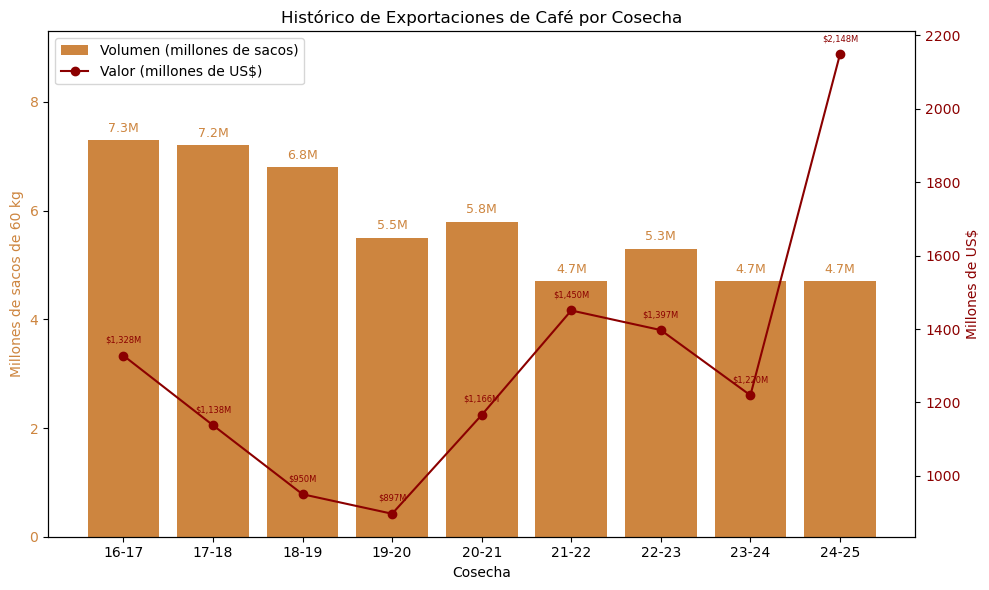
\includegraphics[scale=0.8]{C:/Users/HN32885/Documents/2025/LateX/PPT_Beamer_Sectores/fig1.jpg}
   \end{center}

Honduras pasó de un récord histórico de 7.29 millones de savos exportados en la cosecha 2016-2017 a 4.68 millones de sacos exportados en la cosecha 2023-2024, lo que representa una reducción del 36\%. \textbf{Las exportaciones de café representan el 5\% del PIB nacional y el 20\% del PIB agrícola.} 

  \end{block}
%====================================================
%                                                        BLOQUE 2
%====================================================
  \begin{block}{Bloque 2}

   

  \end{block}
%====================================================
%                                                        BLOQUE 3
%====================================================
  \begin{alertblock}{Bloque 3}



  \end{alertblock}

\end{column}

\separatorcolumn

\begin{column}{\colwidth}
%====================================================
%                                                        BLOQUE 4
%====================================================
  \begin{block}{Bloque 4}



  \end{block}
%====================================================
%                                                        BLOQUE 4
%====================================================
  \begin{block}{Bloque 5}

    \begin{figure}
      \centering
      \begin{tikzpicture}
        \begin{axis}[
            scale only axis,
            no markers,
            domain=0:2*pi,
            samples=100,
            axis lines=center,
            axis line style={-},
            ticks=none]
          \addplot[red] {sin(deg(x))};
          \addplot[blue] {cos(deg(x))};
        \end{axis}
      \end{tikzpicture}
      \caption{Another figure caption.}
    \end{figure}

  \end{block}
%====================================================
%                                                        BLOQUE 6
%====================================================
  \begin{block}{Bloque 6}



  \end{block}

\end{column}

\separatorcolumn

\begin{column}{\colwidth}
%====================================================
%                                                        BLOQUE 7
%====================================================
  \begin{exampleblock}{Bloque 7}

    $$
    \int_{-\infty}^{\infty} e^{-x^2}\,dx = \sqrt{\pi}
    $$


  \end{exampleblock}
%====================================================
%                                                        BLOQUE 8
%====================================================
  \begin{block}{Bloque 8}


    \begin{table}
      \centering
      \begin{tabular}{l r r c}
        \toprule
        \textbf{First column} & \textbf{Second column} & \textbf{Third column} & \textbf{Fourth} \\
        \midrule
        Foo & 13.37 & 384,394 & $\alpha$ \\
        Bar & 2.17 & 1,392 & $\beta$ \\
        Baz & 3.14 & 83,742 & $\delta$ \\
        Qux & 7.59 & 974 & $\gamma$ \\
        \bottomrule
      \end{tabular}
      \caption{A table caption.}
    \end{table}

  \end{block}
%====================================================
%                                                        BLOQUE 9
%====================================================
  \begin{block}{References}

    \nocite{*}
    \footnotesize{\bibliographystyle{plain}\bibliography{poster}}

  \end{block}

\end{column}

\separatorcolumn
\end{columns}
\end{frame}

\end{document}
